\documentclass[11pt]{article}
% Shared preamble for the lecture notes
\usepackage[T1]{fontenc}
\usepackage[utf8]{inputenc}
\usepackage[a4paper,margin=2.4cm]{geometry}
\usepackage{amsmath,amssymb,amsthm,mathtools}
\usepackage{bm}
\usepackage{xcolor}
\usepackage{enumitem}
\usepackage{tikz}
\usetikzlibrary{arrows.meta,positioning,calc}
\usepackage{pgfplots}
\pgfplotsset{compat=1.18}
\usepgfplotslibrary{groupplots}
\usepackage[american]{circuitikz}
\usepackage{microtype}
\usepackage[colorlinks=true,linkcolor=accent,urlcolor=accent,citecolor=accent]{hyperref}
\usepackage{fancyhdr}

\definecolor{accent}{HTML}{B4126B}
\definecolor{accent2}{HTML}{0E7C86}
\definecolor{rule}{HTML}{C9C9D6}

\theoremstyle{definition}
\newtheorem{definition}{Definition}[section]
\newtheorem{example}{Example}[section]
\theoremstyle{plain}
\newtheorem{theorem}{Theorem}[section]
\newtheorem{proposition}[theorem]{Proposition}
\newtheorem{lemma}[theorem]{Lemma}
\newtheorem{corollary}[theorem]{Corollary}
\theoremstyle{remark}
\newtheorem*{remark}{Remark}

% handy macros
\newcommand{\dd}{\mathrm{d}}
\newcommand{\E}{\mathbb{E}}
\newcommand{\R}{\mathbb{R}}
\newcommand{\Var}{\operatorname{Var}}
\newcommand{\Cov}{\operatorname{Cov}}
\newcommand{\KL}{D_{\mathrm{KL}}}
\renewcommand{\vec}[1]{\bm{#1}}
\DeclarePairedDelimiter{\abs}{\lvert}{\rvert}
\DeclarePairedDelimiter{\norm}{\lVert}{\rVert}

\pagestyle{fancy}
\fancyhf{}
\renewcommand{\headrulewidth}{0.4pt}
\fancyhead[L]{\small\itshape Information Theory \& Neural Modeling}
\fancyhead[R]{\small M.\ Vissani}
\fancyfoot[C]{\small\thepage}

% title block
\newcommand{\lectitle}[3]{%
  \begin{center}
    {\footnotesize\sffamily\bfseries\color{accent} GRADUATE LECTURE NOTES \quad\textbullet\quad SCUOLA SUPERIORE SANT'ANNA}\\[2pt]
    {\color{rule}\rule{\linewidth}{0.8pt}}\\[8pt]
    {\LARGE\sffamily\bfseries #1}\\[6pt]
    {\large\sffamily #2}\\[6pt]
    {\small Matteo Vissani \quad\textbullet\quad Course: \emph{Information Theory \& Neural Modeling}}\\[6pt]
    {\color{rule}\rule{\linewidth}{0.8pt}}
  \end{center}
  \vspace{0.6em}
}


\begin{document}
\lectitle{The Integrate-and-Fire Neuron}{Lecture 1 --- From the membrane equation to spiking dynamics and extensions}

\begin{abstract}
\noindent We build the integrate-and-fire (IF) neuron from first principles, with every step of the
derivations worked out, following the treatment of Gerstner, Kistler, Naud \& Paninski,
\emph{Neuronal Dynamics} (EPFL)~\cite{gerstner2014}. We derive the membrane equation from ionic
biophysics, solve the leaky integrate-and-fire (LIF) dynamics in full (integrating factor, Dirac
Green's function, harmonic impedance), obtain the frequency--current relation by explicit
inversion, and treat the noisy neuron through its numerical simulation (the Euler--Maruyama scheme
for stochastic differential equations). We close with a detailed study of the nonlinear and adaptive
extensions --- spike-frequency adaptation, the adaptive exponential model, and the Izhikevich model
and its firing regimes.
\end{abstract}

\tableofcontents
\vspace{1em}

%==================================================================
\section{Biophysical foundations}
%==================================================================

\subsection{The Nernst potential, derived}
A membrane separates two solutions of an ion $s$ (valence $z_s$) at concentrations
$[s]_{\mathrm{in}},[s]_{\mathrm{out}}$. The molar flux density combines Fick diffusion and electric
drift (the Nernst--Planck equation):
\begin{equation}
  J_s=-D_s\frac{\dd c_s}{\dd x}-\frac{z_sF}{RT}\,D_s\,c_s\,\frac{\dd\phi}{\dd x},
\end{equation}
with $D_s$ the diffusivity, $\phi(x)$ the electric potential, $F$ Faraday's constant, $R$ the gas
constant, $T$ temperature. \emph{Step 1 --- equilibrium.} At electrochemical equilibrium the net
flux vanishes, $J_s=0$, so
\begin{equation}
  D_s\frac{\dd c_s}{\dd x}=-\frac{z_sF}{RT}D_s\,c_s\frac{\dd\phi}{\dd x}
  \;\Longrightarrow\;
  \frac{1}{c_s}\frac{\dd c_s}{\dd x}=-\frac{z_sF}{RT}\frac{\dd\phi}{\dd x}.
\end{equation}
\emph{Step 2 --- separate and integrate} across the membrane (from inside to outside):
\begin{equation}
  \int_{[s]_{\mathrm{in}}}^{[s]_{\mathrm{out}}}\frac{\dd c_s}{c_s}
  =-\frac{z_sF}{RT}\int_{\phi_{\mathrm{in}}}^{\phi_{\mathrm{out}}}\dd\phi
  \;\Longrightarrow\;
  \ln\frac{[s]_{\mathrm{out}}}{[s]_{\mathrm{in}}}=-\frac{z_sF}{RT}\big(\phi_{\mathrm{out}}-\phi_{\mathrm{in}}\big).
\end{equation}
\emph{Step 3 --- solve} for the equilibrium membrane potential $E_s\equiv\phi_{\mathrm{in}}-
\phi_{\mathrm{out}}$:
\begin{equation}
  \boxed{\;E_s=\frac{RT}{z_sF}\,\ln\frac{[s]_{\mathrm{out}}}{[s]_{\mathrm{in}}}.\;}
  \label{eq:nernst}
\end{equation}
At $37^\circ$C, $RT/F\approx26.7$\,mV, giving $E_{\mathrm{Na}}\!\approx\!+60$,
$E_{\mathrm{K}}\!\approx\!-90$, $E_{\mathrm{Cl}}\!\approx\!-65$\,mV.

\subsection{Leak, capacitance, and current balance}
Near rest the many background conductances combine into a single Ohmic \emph{leak}
$I_L=g_L(V-E_L)$ with $E_L\approx V_{\mathrm{rest}}$~\cite{gerstner2014,dayan2001}. The bilayer stores
charge $Q=C_mV$; differentiating gives the capacitive current $I_C=\dd Q/\dd t=C_m\,\dd V/\dd t$.
Treating the soma as isopotential, charge conservation at the node (Kirchhoff) reads
\begin{equation}
  C_m\frac{\dd V}{\dd t}=-I_{\mathrm{ion}}(V,t)+I(t).
  \label{eq:kcl}
\end{equation}

\begin{figure}[h]
\centering
\begin{circuitikz}[line width=0.85pt, scale=1.0]
  \draw (0,0) -- (6.2,0);
  \draw (0,3) -- (6.2,3);
  \draw (1,3) to[C, l_=$C_m$] (1,0);
  \draw (3,3) to[R, l=$R{=}1/g_L$] (3,1.55) to[battery1, l=$E_L$] (3,0);
  \draw (5.2,0) to[isource, l=$I(t)$] (5.2,3);
  \node[circ] at (1,3){}; \node[circ] at (3,3){}; \node[circ] at (5.2,3){};
  \node[circ] at (1,0){}; \node[circ] at (3,0){}; \node[circ] at (5.2,0){};
  \node[above] at (3,3.15) {\small inside\ \ ($V$)};
  \node[below] at (3,-0.15) {\small outside (ground)};
\end{circuitikz}
\caption{Equivalent circuit of an isopotential membrane patch (cf.~\cite{gerstner2014}, Ch.~1). The
injected current $I(t)$ points \emph{into} the intracellular node; the leak branch is $R=1/g_L$ in
series with the reversal battery $E_L$.}
\end{figure}

\subsection{From Hodgkin--Huxley to integrate-and-fire}
The full biophysics of spike generation is the Hodgkin--Huxley (HH) model, in which the ionic
current is the sum of voltage-gated sodium, potassium, and leak currents:
\begin{equation}
  C_m\dot V=-\bar g_{\mathrm{Na}}m^3h(V-E_{\mathrm{Na}})-\bar g_{\mathrm K}n^4(V-E_{\mathrm K})
            -g_L(V-E_L)+I(t),
\end{equation}
with gating variables $x\in\{m,h,n\}$ each obeying $\dot x=\alpha_x(V)(1-x)-\beta_x(V)\,x$. Sodium
activation $m$ is fast and regenerative: past a threshold it opens explosively, producing the
upstroke; then inactivation $h$ and the potassium variable $n$ repolarize and transiently
hyperpolarize the cell (the refractory period). Two facts license the IF reduction: (i) the spike
is \emph{stereotyped}, so its waveform carries little information and may be replaced by an event
plus a reset; (ii) \emph{between} spikes the dynamics are nearly linear, set by the leak. Discarding
the spike shape and keeping the subthreshold leak yields exactly the LIF equation below with a
threshold and reset --- the IF neuron is the analytic \emph{caricature} of HH. The exponential and
quadratic models of \S\ref{sec:adex} restore an approximation of the sodium upstroke.

\subsection{The cable equation and the isopotential assumption}
Real neurons are spatially extended. Treating a dendrite as a thin cable of radius $a$ and axial
resistivity $r_i$, current conservation gives the \textbf{cable equation}
\begin{equation}
  c_m\,\partial_t V=\frac{a}{2r_i}\,\partial_x^2 V-i_{\mathrm{ion}}(V)+i_{\mathrm{ext}}(x,t),
\end{equation}
a reaction--diffusion PDE whose electrotonic length constant $\lambda=\sqrt{aR_m/2r_i}$ sets how far
voltage spreads. When the cell is small compared with $\lambda$ (or we lump it into one
compartment) the diffusion term $\partial_x^2V$ is negligible and the PDE collapses to the single
ODE \eqref{eq:kcl}: this \emph{isopotential} assumption is what we use throughout. Multi-compartment
models reinstate $\partial_x^2V$ to capture dendritic processing.

%==================================================================
\section{The leaky integrate-and-fire model}
%==================================================================
Keeping only the leak, $I_{\mathrm{ion}}=g_L(V-E_L)$, equation \eqref{eq:kcl} reads
$C_m\dot V=-g_L(V-E_L)+I(t)$. \emph{Dividing through by $g_L$},
\begin{equation}
  \frac{C_m}{g_L}\frac{\dd V}{\dd t}=-(V-E_L)+\frac{I(t)}{g_L},
\end{equation}
and \emph{defining} the membrane time constant $\tau_m\coloneqq C_m/g_L$ and resistance
$R\coloneqq 1/g_L$ (so $\tau_m=RC_m$),
\begin{equation}
  \boxed{\;\tau_m\frac{\dd V}{\dd t}=-(V-E_L)+R\,I(t).\;}
  \label{eq:lif}
\end{equation}
This passive integrator cannot spike; we add the \textbf{fire-and-reset} rule
\begin{equation}
  V(t^-)=\vartheta\;\Rightarrow\;\text{spike at }t,\quad V(t^+)=V_r,
  \label{eq:reset}
\end{equation}
(threshold $\vartheta$, reset $V_r$, optional refractory $\tau_{\mathrm{ref}}$). The LIF is a
\emph{hybrid} system: smooth linear flow \eqref{eq:lif} interrupted by the discrete map
\eqref{eq:reset} (Fig.~\ref{fig:trace}).

\begin{figure}[h]
\centering
\begin{tikzpicture}
\begin{groupplot}[group style={group size=1 by 2, vertical sep=0.9cm}, width=13cm, height=3.6cm,
  axis lines=left, xmin=0, xmax=6, enlarge x limits=false,
  tick label style={font=\scriptsize}, label style={font=\small}]
\nextgroupplot[ylabel={$I(t)$}, ymin=-0.1, ymax=2, xticklabels={}, ytick={0,1.5}]
  \addplot[accent2, very thick, const plot, mark=none] coordinates {(0,0)(0.5,0)(0.5,1.5)(6,1.5)};
\nextgroupplot[ylabel={$V(t)$}, xlabel={time $\;t/\tau_m$}, ymin=0, ymax=2.25,
  ytick={0,1,1.5}, yticklabels={$V_r$,$\vartheta$,{}}, clip=false]
  \addplot[gray, densely dotted, domain=0:6]{1.5};
  \node[anchor=east, font=\scriptsize, gray] at (axis cs:6,1.72){asymptote $E_L{+}RI_0$};
  \addplot[gray, dashed, domain=0:6]{1};
  \addplot[accent, very thick] table {sim_step.dat};
  \addplot[accent, very thick] coordinates {(1.6,1)(1.6,1.45)};
  \addplot[accent, very thick] coordinates {(2.7,1)(2.7,1.45)};
  \addplot[accent, very thick] coordinates {(3.8,1)(3.8,1.45)};
  \addplot[accent, very thick] coordinates {(4.9,1)(4.9,1.45)};
  \addplot[accent, very thick] coordinates {(6.0,1)(6.0,1.45)};
  \node[font=\scriptsize, accent2, anchor=west] at (axis cs:0.95,0.45){(1) charge};
  \node[font=\scriptsize, anchor=south] at (axis cs:1.6,1.55){(2) spike};
  \draw[-{Latex[length=1.6mm]}, black!70] (axis cs:1.9,1.0) to[bend left=25] (axis cs:1.62,0.08);
  \node[font=\scriptsize, anchor=west] at (axis cs:1.95,0.78){(3) reset};
\end{groupplot}
\end{tikzpicture}
\caption{LIF response to a constant step current. \emph{Top}: $I(t)$ switched on at
$t=0.5\,\tau_m$. \emph{Bottom}: the membrane potential (1)~\emph{charges} exponentially toward the
asymptote $E_L+RI_0$ (dotted), (2)~hits the threshold $\vartheta$ (dashed) and \emph{fires} a spike
(vertical mark), then (3)~\emph{resets} to $V_r$; the cycle repeats with period
$T=\tau_m\ln\frac{E_L+RI_0-V_r}{E_L+RI_0-\vartheta}$. Cf.~\cite{gerstner2014}, \S1.3.}
\label{fig:trace}
\end{figure}

\paragraph{How to read Fig.~\ref{fig:trace} (worked walk-through).}
Before the current is injected the cell sits at rest, $V=E_L=V_r$ (flat line). When the step turns
on, the right-hand side of \eqref{eq:lif} becomes positive, so $\dd V/\dd t>0$ and $V$ rises. It
would relax exponentially toward the \emph{asymptote} $E_L+RI_0$ (the value at which leak and input
currents balance), but here that asymptote ($1.5$) lies \emph{above} the threshold ($1$): the
potential never gets there. Instead, when $V$ reaches $\vartheta$ the fire-and-reset rule
\eqref{eq:reset} triggers --- we mark a spike and instantaneously set $V\!\to\!V_r$ --- and the
charging starts over. Because the drive is constant, every cycle is identical, so the neuron fires
\emph{periodically} with the interval $T$ derived in \eqref{eq:isi}. Two limits are worth noting for
students: if the asymptote were \emph{below} threshold ($E_L+RI_0<\vartheta$) the neuron would
charge up, stall below $\vartheta$, and never fire (sub-rheobase); the closer the asymptote sits to
$\vartheta$, the slower the final approach and the longer $T$ --- this is the origin of the
arbitrarily low firing rates near rheobase.

\paragraph{A geometric picture: the phase line.}
A second way to see the same dynamics is to plot the \emph{rate of change} $\dd V/\dd t$ against
$V$ itself (Fig.~\ref{fig:phaseline}). For the LIF this is the straight line $\dd V/\dd t=
[\,(E_L+RI_0)-V\,]/\tau_m$: positive when $V$ is below the asymptote (so $V$ moves right) and zero
at the asymptote. The flow therefore pushes $V$ rightward, but the threshold $\vartheta$ acts as a
trap-door before the asymptote is reached: upon contact, $V$ is teleported back to $V_r$ and the
motion repeats. This phase-line view is what generalizes to the nonlinear models of
\S\ref{sec:adex}, where the straight line becomes curved and can create or destroy fixed points.

\begin{figure}[h]
\centering
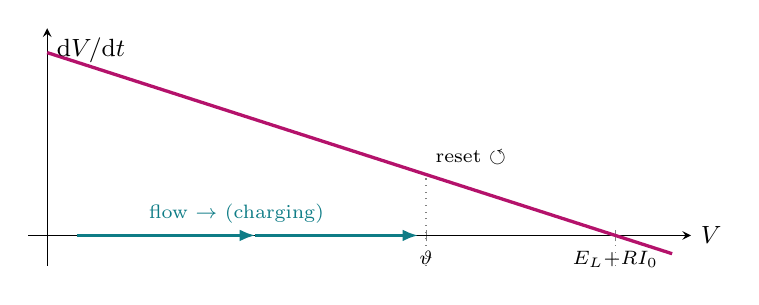
\begin{tikzpicture}
\begin{axis}[width=10cm, height=4.6cm, axis lines=middle, xlabel={$V$}, ylabel={$\dd V/\dd t$},
  xmin=-0.05, xmax=1.7, ymin=-0.25, ymax=1.7, xtick={0,1,1.5}, xticklabels={$V_r$,$\vartheta$,$E_L{+}RI_0$},
  ytick=\empty, x label style={anchor=west}, tick label style={font=\scriptsize}, label style={font=\small}]
  \addplot[accent, very thick, domain=0:1.65]{1.5-x};
  \addplot[black!50, dotted] coordinates {(1,-0.25)(1,0.5)};
  \addplot[black!50, dotted] coordinates {(1.5,-0.25)(1.5,0.05)};
  % flow arrows along V axis (V increases because dV/dt>0)
  \draw[-{Latex[length=2mm]}, accent2, very thick] (axis cs:0.08,0)--(axis cs:0.55,0);
  \draw[-{Latex[length=2mm]}, accent2, very thick] (axis cs:0.55,0)--(axis cs:0.98,0);
  \node[font=\scriptsize, accent2, anchor=south] at (axis cs:0.5,0.02){flow $\to$ (charging)};
  \node[font=\scriptsize, anchor=south west] at (axis cs:1.0,0.5){reset $\circlearrowleft$};
\end{axis}
\end{tikzpicture}
\caption{Phase line of the LIF: $\dd V/\dd t$ versus $V$. The flow (arrows) carries $V$ toward the
asymptote $E_L+RI_0$ where $\dd V/\dd t=0$, but the threshold $\vartheta$ intercepts it first and
resets it to $V_r$ (curved arrow). When $E_L+RI_0<\vartheta$ the line crosses zero before
$\vartheta$ and the neuron settles silently (sub-rheobase).}
\label{fig:phaseline}
\end{figure}

%==================================================================
\section{Subthreshold dynamics, derived in full}
%==================================================================

\subsection{General solution by the integrating factor}
Rewrite \eqref{eq:lif} in standard linear form by dividing by $\tau_m$:
\begin{equation}
  \frac{\dd V}{\dd t}+\frac{1}{\tau_m}V=\frac{1}{\tau_m}\big(E_L+RI(t)\big).
\end{equation}
\emph{Step 1 --- integrating factor.} Multiply both sides by $\mu(t)=e^{t/\tau_m}$. The left side
becomes an exact derivative because $\frac{\dd}{\dd t}\!\big(e^{t/\tau_m}V\big)=e^{t/\tau_m}\dot V+
\frac{1}{\tau_m}e^{t/\tau_m}V$:
\begin{equation}
  \frac{\dd}{\dd t}\Big(e^{t/\tau_m}V\Big)=\frac{1}{\tau_m}e^{t/\tau_m}\big(E_L+RI(t)\big).
\end{equation}
\emph{Step 2 --- integrate} from $t_0$ to $t$:
\begin{equation}
  e^{t/\tau_m}V(t)-e^{t_0/\tau_m}V(t_0)
   =\frac{1}{\tau_m}\int_{t_0}^t e^{s/\tau_m}\big(E_L+RI(s)\big)\,\dd s.
\end{equation}
\emph{Step 3 --- evaluate the $E_L$ piece}: $\frac{E_L}{\tau_m}\int_{t_0}^t e^{s/\tau_m}\dd s
=E_L\big(e^{t/\tau_m}-e^{t_0/\tau_m}\big)$. \emph{Step 4 --- divide by $e^{t/\tau_m}$} and use
$R/\tau_m=1/C_m$:
\begin{equation}
  \boxed{\;V(t)=E_L+\big(V(t_0)-E_L\big)e^{-(t-t_0)/\tau_m}
   +\frac{1}{C_m}\int_{t_0}^t e^{-(t-s)/\tau_m}I(s)\,\dd s.\;}
  \label{eq:gensol}
\end{equation}

\subsection{Dirac impulse and the Green's function}
Take the input to be a charge $q$ delivered instantaneously, $I(t)=q\,\delta(t)$, with the cell at
rest before $t=0$ ($t_0\to-\infty$, $V(t_0)=E_L$). The convolution term in \eqref{eq:gensol} is
evaluated with the \emph{sifting property} $\int f(s)\delta(s-a)\dd s=f(a)$:
\begin{equation}
  V(t)-E_L=\frac{1}{C_m}\int_{-\infty}^{t} e^{-(t-s)/\tau_m}\,q\,\delta(s)\,\dd s
   =\frac{q}{C_m}\,e^{-t/\tau_m}\quad(t>0).
\end{equation}
Hence the potential \emph{jumps} by $q/C_m$ at $t=0$ and relaxes exponentially. Writing
$V(t)-E_L=q\,\kappa(t)$ identifies the \textbf{Green's function} (impulse response / elementary PSP)
\begin{equation}
  \kappa(t)=\frac{1}{C_m}\,e^{-t/\tau_m}\,\Theta(t),
  \label{eq:green}
\end{equation}
and by linearity the response to \emph{any} input is the convolution
\begin{equation}
  V(t)=E_L+(\kappa*I)(t)=E_L+\int_{-\infty}^t\kappa(t-s)I(s)\,\dd s :
  \label{eq:conv}
\end{equation}
the LIF membrane is a first-order low-pass filter.

\begin{figure}[h]
\centering
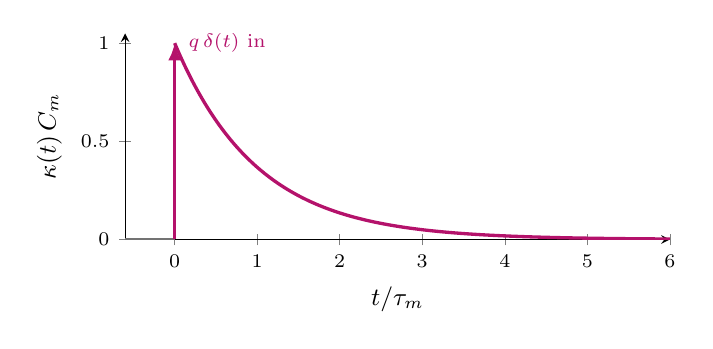
\begin{tikzpicture}
\begin{axis}[width=8.5cm, height=4.2cm, axis lines=left, xlabel={$t/\tau_m$},
  ylabel={$\kappa(t)\,C_m$}, ymin=0, ymax=1.05, xmin=-0.6, xmax=6,
  tick label style={font=\scriptsize}, label style={font=\small}]
  \addplot[black!55, very thick] coordinates {(-0.6,0)(0,0)};
  \draw[-{Latex[length=2.2mm]}, accent, very thick] (axis cs:0,0) -- (axis cs:0,1);
  \node[accent, font=\scriptsize, anchor=west] at (axis cs:0.05,1.0){$q\,\delta(t)$ in};
  \addplot[accent, very thick, domain=0:6, samples=200]{exp(-x)};
\end{axis}
\end{tikzpicture}
\caption{Green's function \eqref{eq:green}: response to a Dirac impulse $q\,\delta(t)$ --- a jump
followed by $e^{-t/\tau_m}$ decay (the elementary postsynaptic potential).}
\label{fig:epsp}
\end{figure}

\paragraph{Temporal summation: integrating inputs.}
Because the membrane is linear \eqref{eq:conv}, the response to a train of synaptic pulses is the
\emph{sum} of the individual postsynaptic potentials of Fig.~\ref{fig:epsp}. This is the
``integrate'' in integrate-and-fire. Figure~\ref{fig:summation} simulates a neuron receiving brief
inputs (arrows): \emph{isolated} inputs (at $t=1,3$) each produce a PSP that simply decays away, but
a \emph{rapid burst} of inputs arriving within roughly one time constant \emph{summate} --- each new
PSP rides on the tail of the previous one --- until the accumulated depolarization crosses
$\vartheta$ and the neuron fires. The neuron thus acts as a leaky coincidence detector: inputs that
are clustered in time are far more effective than the same inputs spread out, because the leak
forgets the early ones.

\begin{figure}[h]
\centering
\begin{tikzpicture}
\begin{axis}[width=13cm, height=4.4cm, axis lines=left, xlabel={time $\;t/\tau_m$}, ylabel={$V(t)$},
  xmin=0, xmax=9, ymin=-0.32, ymax=1.2, ytick={0,1}, yticklabels={$V_r$,$\vartheta$},
  tick label style={font=\scriptsize}, label style={font=\small}]
  \addplot[gray, dashed, domain=0:9]{1};
  \addplot[accent, very thick] table {sim_sum.dat};
  \draw[-{Latex[length=1.8mm]}, accent2, thick] (axis cs:1.0,-0.27)--(axis cs:1.0,-0.04);
  \draw[-{Latex[length=1.8mm]}, accent2, thick] (axis cs:3.0,-0.27)--(axis cs:3.0,-0.04);
  \draw[-{Latex[length=1.8mm]}, accent2, thick] (axis cs:4.8,-0.27)--(axis cs:4.8,-0.04);
  \draw[-{Latex[length=1.8mm]}, accent2, thick] (axis cs:5.2,-0.27)--(axis cs:5.2,-0.04);
  \draw[-{Latex[length=1.8mm]}, accent2, thick] (axis cs:5.6,-0.27)--(axis cs:5.6,-0.04);
  \draw[-{Latex[length=1.8mm]}, accent2, thick] (axis cs:6.0,-0.27)--(axis cs:6.0,-0.04);
  \draw[-{Latex[length=1.8mm]}, accent2, thick] (axis cs:6.4,-0.27)--(axis cs:6.4,-0.04);
  \node[font=\scriptsize, accent2, anchor=west] at (axis cs:0.05,-0.27){synaptic inputs};
\end{axis}
\end{tikzpicture}
\caption{Temporal summation (simulated LIF with delta inputs, $\tau_m=1$). Isolated inputs decay
without effect; the fast cluster near $t\!\approx\!5$--$6$ summates past $\vartheta$ and triggers a
spike, after which $V$ resets. The leak makes the neuron sensitive to input \emph{timing}.}
\label{fig:summation}
\end{figure}

\subsection{Step response, derived}
For a current step $I(t)=I_0\,\Theta(t)$ with $V(0)=V_0$, evaluate the convolution integral in
\eqref{eq:gensol} explicitly:
\begin{align}
  \frac{1}{C_m}\int_0^t e^{-(t-s)/\tau_m}I_0\,\dd s
  &=\frac{I_0}{C_m}\,e^{-t/\tau_m}\int_0^t e^{s/\tau_m}\dd s
   =\frac{I_0}{C_m}\,e^{-t/\tau_m}\,\tau_m\big(e^{t/\tau_m}-1\big)\notag\\
  &=\frac{I_0\tau_m}{C_m}\big(1-e^{-t/\tau_m}\big)=RI_0\big(1-e^{-t/\tau_m}\big),
\end{align}
using $\tau_m/C_m=R$. Therefore
\begin{equation}
  V(t)=V_\infty+(V_0-V_\infty)\,e^{-t/\tau_m},\qquad V_\infty=E_L+RI_0,
  \label{eq:step}
\end{equation}
the smooth charging curve of Fig.~\ref{fig:trace}.

\subsection{Harmonic response: impedance, derived}
Seek the stationary response to $I(t)=I_0e^{i\omega t}$ with the ansatz $V(t)-E_L=Z(\omega)I_0
e^{i\omega t}$. Substitute into \eqref{eq:lif} (in the form $\tau_m\dot V+(V-E_L)=RI$):
\begin{equation}
  \tau_m\,(i\omega)Z I_0e^{i\omega t}+Z I_0e^{i\omega t}=R\,I_0e^{i\omega t}
  \;\Longrightarrow\;Z(\omega)\,(1+i\omega\tau_m)=R,
\end{equation}
so $Z(\omega)=R/(1+i\omega\tau_m)$. \emph{Rationalize} (multiply by the conjugate) to read off
modulus and phase:
\begin{equation}
  Z(\omega)=\frac{R(1-i\omega\tau_m)}{1+(\omega\tau_m)^2},\quad
  \abs{Z(\omega)}=\frac{R}{\sqrt{1+(\omega\tau_m)^2}},\quad
  \arg Z(\omega)=-\arctan(\omega\tau_m).
  \label{eq:Z}
\end{equation}
The amplitude is flat below the cutoff $f_c=1/(2\pi\tau_m)$ and falls as $1/\omega$ above it; the
phase lags from $0^\circ$ to $-90^\circ$ (Fig.~\ref{fig:bode}). The passive LIF has no resonance.

\begin{figure}[h]
\centering
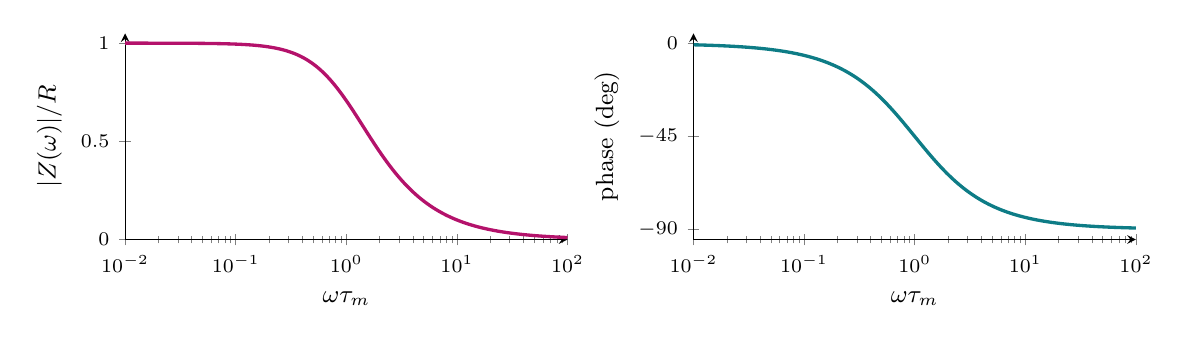
\begin{tikzpicture}
\begin{groupplot}[group style={group size=2 by 1, horizontal sep=1.6cm}, width=7.2cm, height=4.2cm,
  xmode=log, axis lines=left, xlabel={$\omega\tau_m$}, xmin=0.01, xmax=100,
  tick label style={font=\scriptsize}, label style={font=\small}]
\nextgroupplot[ylabel={$|Z(\omega)|/R$}, ymin=0, ymax=1.05, domain=0.01:100, samples=200]
  \addplot[accent, very thick]{1/sqrt(1+x^2)};
\nextgroupplot[ylabel={phase (deg)}, ymin=-95, ymax=5, ytick={0,-45,-90}, domain=0.01:100, samples=200]
  \addplot[accent2, very thick]{-atan(x)};
\end{groupplot}
\end{tikzpicture}
\caption{Bode diagram of the membrane filter \eqref{eq:Z}: amplitude (left) and phase (right).}
\label{fig:bode}
\end{figure}

%==================================================================
\section{Deterministic firing and the $f$--$I$ curve, derived}
%==================================================================
With constant supra-threshold drive the trajectory between resets starts at $V(0)=V_r$ and follows
\eqref{eq:step}, $V(t)=V_\infty+(V_r-V_\infty)e^{-t/\tau_m}$. \emph{Impose the threshold condition}
$V(T)=\vartheta$ and solve for the interval $T$:
\begin{align}
  \vartheta&=V_\infty+(V_r-V_\infty)e^{-T/\tau_m}
   \;\Longrightarrow\;
   e^{-T/\tau_m}=\frac{\vartheta-V_\infty}{V_r-V_\infty}=\frac{V_\infty-\vartheta}{V_\infty-V_r},\notag\\
  T&=\tau_m\ln\frac{V_\infty-V_r}{V_\infty-\vartheta}
   =\tau_m\ln\frac{RI_0+E_L-V_r}{RI_0+E_L-\vartheta}.
  \label{eq:isi}
\end{align}
Adding the refractory period, the rate is $r=1/(\tau_{\mathrm{ref}}+T)$:
\begin{equation}
  \boxed{\;r(I_0)=\Big[\tau_{\mathrm{ref}}+\tau_m\ln\frac{RI_0+E_L-V_r}{RI_0+E_L-\vartheta}\Big]^{-1},
  \quad I_0>I_{\mathrm{rh}}.\;}
  \label{eq:fI}
\end{equation}
\emph{Rheobase}: the argument of the logarithm diverges (so $T\to\infty$, $r\to0$) when
$RI_0+E_L=\vartheta$, i.e.\ at $I_{\mathrm{rh}}=(\vartheta-E_L)/R$. \emph{Strong drive}: expanding
$\ln\frac{V_\infty-V_r}{V_\infty-\vartheta}=\ln\!\big(1+\frac{\vartheta-V_r}{V_\infty-\vartheta}\big)
\approx\frac{\vartheta-V_r}{V_\infty}$ for $V_\infty\gg\vartheta$ gives $r\approx
RI_0/[\tau_m(\vartheta-V_r)]$, saturating at $1/\tau_{\mathrm{ref}}$.

\begin{figure}[h]
\centering
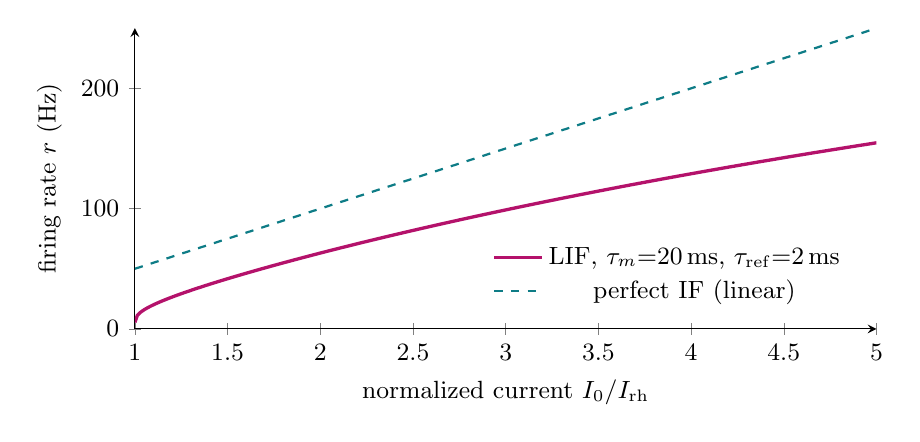
\begin{tikzpicture}
\begin{axis}[width=11cm,height=5.4cm, axis lines=left,
  xlabel={normalized current $I_0/I_{\mathrm{rh}}$}, ylabel={firing rate $r$ (Hz)},
  domain=1.0001:5, samples=300, ymin=0, xmin=1, xmax=5,
  legend style={font=\small,draw=none,at={(0.97,0.05)},anchor=south east},
  tick label style={font=\small}, label style={font=\small}]
  \addplot[accent, very thick]{1/(0.002+0.02*ln(x/(x-1)))};
  \addlegendentry{LIF, $\tau_m{=}20$\,ms, $\tau_{\mathrm{ref}}{=}2$\,ms}
  \addplot[accent2, thick, dashed]{x/0.02};
  \addlegendentry{perfect IF (linear)}
\end{axis}
\end{tikzpicture}
\caption{The $f$--$I$ relation \eqref{eq:fI}: continuous onset at rheobase, saturation toward
$1/\tau_{\mathrm{ref}}$ (solid); perfect IF is linear (dashed). Cf.~\cite{gerstner2014,burkitt2006}.}
\end{figure}

%==================================================================
\section{Spike trains as Dirac combs}
%==================================================================
A spike train is fully specified by its firing times $\{t_f\}$ through the spike-train density
\begin{equation}
  \rho(t)=\sum_f\delta(t-t_f),
  \label{eq:comb}
\end{equation}
whose expectation is the instantaneous rate $\nu(t)=\langle\rho(t)\rangle$ and whose integral over a
window is the spike count. Synaptic input is this comb filtered by a synaptic kernel $\alpha$:
$I_{\mathrm{syn}}=q(\alpha*\rho)$, so by \eqref{eq:conv} the voltage is a sum of postsynaptic
potentials $V(t)-E_L=q\sum_f(\kappa*\alpha)(t-t_f)$, the spike-response picture of~\S\ref{sec:srm}.

\begin{figure}[h]
\centering
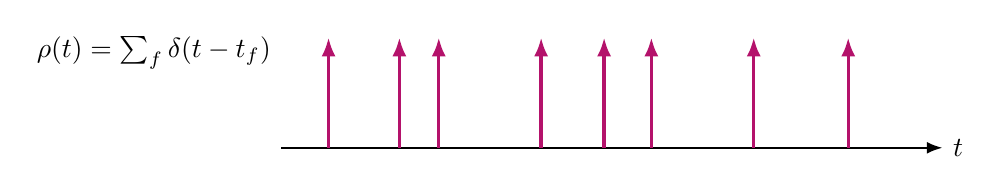
\begin{tikzpicture}[line width=0.9pt]
  \draw[-{Latex[length=2mm]}] (0,0)--(8.4,0) node[right]{$t$};
  \foreach \x in {0.6,1.5,2.0,3.3,4.1,4.7,6.0,7.2} {
    \draw[-{Latex[length=2.4mm]}, accent, very thick] (\x,0)--(\x,1.4);}
  \node[anchor=east] at (0,1.2) {$\rho(t)=\sum_f\delta(t-t_f)$};
\end{tikzpicture}
\caption{A spike train as a sum of Dirac deltas (a Dirac comb); each arrow marks a firing time.}
\end{figure}

Under constant drive the LIF fires periodically ($C_V=0$), unlike cortical neurons ($C_V\approx1$):
irregularity comes from input fluctuations, derived next~\cite{gerstner2014,brunel2000}.

%==================================================================
\section{The noisy neuron and its numerical simulation}
%==================================================================

\subsection{From synaptic bombardment to a stochastic equation}
A cortical neuron receives thousands of synaptic inputs. Modelling their net effect as a mean drive
$\mu$ plus Gaussian fluctuations of intensity $\sigma$ (justified when inputs are many, small, and
fast), the LIF equation \eqref{eq:lif} becomes the \textbf{Langevin equation}
\begin{equation}
  \tau_m\,\dd V=\big[-(V-E_L)+\mu\big]\dd t+\sigma\sqrt{\tau_m}\,\dd W_t,
  \label{eq:ou}
\end{equation}
where $W_t$ is a Wiener process (Brownian motion: $\dd W_t$ is Gaussian, zero-mean, with
$\langle\dd W_t^2\rangle=\dd t$), together with the reset rule \eqref{eq:reset}. This is a
\emph{stochastic differential equation} (SDE): we cannot integrate it by hand for each realization,
so we simulate it.

\subsection{Numerical integration: the Euler--Maruyama method}
The standard scheme for an SDE is \textbf{Euler--Maruyama}, the stochastic analogue of forward
Euler. Discretize time into steps $\Delta t$, write $V_k\approx V(k\Delta t)$, and update
\begin{equation}
  \boxed{\;V_{k+1}=V_k+\frac{1}{\tau_m}\big[-(V_k-E_L)+\mu\big]\Delta t
   \;+\;\frac{\sigma}{\sqrt{\tau_m}}\,\sqrt{\Delta t}\;\xi_k,\qquad
   \xi_k\sim\mathcal N(0,1)\ \text{i.i.d.}\;}
  \label{eq:em}
\end{equation}
The one feature that distinguishes this from a deterministic Euler step is that \textbf{the noise
term scales as $\sqrt{\Delta t}$, not $\Delta t$}. The reason: over a step the Wiener increment
$\Delta W=W_{k+1}-W_k$ is Gaussian with variance $\Delta t$, so $\Delta W=\sqrt{\Delta t}\,\xi_k$.
(Writing $\Delta t$ instead of $\sqrt{\Delta t}$ is a common bug --- it makes the noise vanish as
$\Delta t\to0$.) The spike rule is checked after each update:
\begin{center}
\fbox{\parbox{0.92\linewidth}{\small
\textbf{Algorithm (noisy LIF by Euler--Maruyama).}\\
choose $\Delta t\ll\tau_m$;\quad set $V_0=V_r$, spike list empty.\\
for $k=0,1,2,\dots$:\\
\quad draw $\xi_k\sim\mathcal N(0,1)$ and update $V_{k+1}$ via \eqref{eq:em};\\
\quad if $V_{k+1}\ge\vartheta$:\ record a spike at $t=(k{+}1)\Delta t$ and set $V_{k+1}\leftarrow V_r$.
}}
\end{center}
Euler--Maruyama has \emph{strong} order $\tfrac12$ and \emph{weak} order $1$ in $\Delta t$; in
practice take $\Delta t$ a small fraction of $\tau_m$ (e.g.\ $\Delta t\le\tau_m/50$) and confirm the
results do not change when $\Delta t$ is halved. Every quantity of interest is then \emph{measured}
from the simulated trajectories rather than computed from any analytic formula: the firing rate as
(number of spikes)$/$(time), the $C_V$ from the inter-spike intervals, and the membrane-potential
distribution as a histogram of the subthreshold $V_k$ (Figs.~\ref{fig:vdist}--\ref{fig:fInoise}).
This Monte-Carlo recipe needs no heavy probability machinery and applies unchanged to the nonlinear
models below, for which closed-form firing rates do not exist.

\paragraph{The key qualitative result.} With a \emph{subthreshold} mean drive ($\mu<\vartheta-E_L$)
the deterministic neuron is silent, but the fluctuations occasionally push $V$ across $\vartheta$,
producing \emph{irregular} firing ($C_V\approx1$). Noise therefore smooths the $f$--$I$ curve and
abolishes the hard rheobase --- the \emph{fluctuation-driven} regime in which real cortical and
subcortical neurons operate.

\paragraph{The membrane-potential distribution.} Histogramming the subthreshold voltage $V_k$ from a
long Euler--Maruyama run gives the membrane-potential distribution $p_0(V)$ (Fig.~\ref{fig:vdist}):
it peaks near the mean drive and falls to zero at the threshold $\vartheta$, because every
trajectory that reaches $\vartheta$ is reset to $V_r$. How often that happens is exactly the firing
rate --- which here we simply count from the simulation.

\begin{figure}[h]
\centering
\begin{tikzpicture}
\begin{axis}[width=10cm, height=4cm, axis lines=left, xlabel={membrane potential $V$},
  ylabel={density $p_0(V)$}, xmin=-1.1, xmax=1.05, ymin=0, ytick=\empty,
  tick label style={font=\scriptsize}, label style={font=\small}]
  \addplot[accent, very thick] table {Vhist.dat};
  \addplot[gray, dashed] coordinates {(1,0)(1,2.2)};
  \node[anchor=south east, font=\scriptsize, gray] at (axis cs:1.0,1.6){$\vartheta$ (reset)};
\end{axis}
\end{tikzpicture}
\caption{Membrane-potential distribution under noise, as a histogram of the subthreshold voltage
from a long Euler--Maruyama simulation of \eqref{eq:ou}. It peaks near the mean drive and vanishes
at $\vartheta$ (every trajectory reaching threshold is reset to $V_r$).}
\label{fig:vdist}
\end{figure}

\paragraph{What the noise does, in pictures.} Figure~\ref{fig:noisy} is a single Euler--Maruyama
trajectory with subthreshold mean drive: the deterministic neuron would be silent, yet fluctuations
push $V$ across $\vartheta$ at irregular times. Counting spikes as the mean drive is varied gives
the $f$--$I$ curve of Fig.~\ref{fig:fInoise}: the deterministic curve has a sharp rheobase corner,
while noise rounds it off and yields a nonzero rate even below threshold.

\begin{figure}[h]
\centering
\begin{tikzpicture}
\begin{axis}[width=13cm, height=4.2cm, axis lines=left, xlabel={time $\;t/\tau_m$}, ylabel={$V(t)$},
  xmin=0, xmax=18, ymin=-0.25, ymax=1.5, ytick={0,1}, yticklabels={$V_r$,$\vartheta$},
  tick label style={font=\scriptsize}, label style={font=\small}]
  \addplot[gray, dashed, domain=0:18]{1};
  \addplot[accent, thick] table {sim_noisy.dat};
  \addplot[only marks, mark=*, mark size=1.1pt, accent2] table {sim_noisy_sp.dat};
\end{axis}
\end{tikzpicture}
\caption{Fluctuation-driven firing (Euler--Maruyama simulation of \eqref{eq:ou}, mean drive
$\mu=0.92\,\vartheta$, below rheobase). Subthreshold fluctuations occasionally cross $\vartheta$
(dots), giving \emph{irregular} spikes ($C_V\approx1$), unlike the clockwork firing of
Fig.~\ref{fig:trace}.}
\label{fig:noisy}
\end{figure}

\begin{figure}[h]
\centering
\begin{tikzpicture}
\begin{axis}[width=11cm, height=5cm, axis lines=left, xlabel={mean drive $\mu/(\vartheta-E_L)$},
  ylabel={firing rate $r\,\tau_m$}, xmin=0.5, xmax=3, ymin=0,
  legend style={font=\small, draw=none, at={(0.03,0.97)}, anchor=north west},
  tick label style={font=\small}, label style={font=\small}]
  \addplot[accent2, thick, dashed] table {fI_det.dat}; \addlegendentry{deterministic ($\sigma=0$)}
  \addplot[accent, very thick] table {fI_noise.dat};   \addlegendentry{with noise ($\sigma=0.3$)}
  \draw[gray, dotted] (axis cs:1,0)--(axis cs:1,0.9);
  \node[font=\scriptsize, gray, anchor=south] at (axis cs:1,0.9){rheobase};
\end{axis}
\end{tikzpicture}
\caption{Noise smooths the $f$--$I$ curve, here \emph{measured by Euler--Maruyama Monte-Carlo}
(spikes counted over a long simulation at each $\mu$). The deterministic curve (dashed) is exactly
zero below the rheobase ($\mu=\vartheta$) and rises with a sharp corner; noise (solid) rounds the
corner and gives a nonzero rate even for subthreshold mean drive.}
\label{fig:fInoise}
\end{figure}

%==================================================================
\section{Nonlinear and adaptive extensions}\label{sec:adex}
%==================================================================

\subsection{Quadratic IF and the theta neuron}
Expanding the spike nonlinearity to quadratic order gives $\tau_m\dot V=a(V-V_r)(V-V_c)+RI$, the
normal form of a saddle-node-on-invariant-circle (SNIC) bifurcation. The substitution
$V=\tan(\theta/2)$ (so $\dot V=\tfrac12\sec^2(\theta/2)\,\dot\theta$ and $1+V^2=\sec^2(\theta/2)$)
maps it to the \textbf{theta neuron} $\dot\theta=(1-\cos\theta)+(1+\cos\theta)\,I$ on the circle ---
the canonical Type-I oscillator with $r\propto\sqrt{I-I_c}$ near onset.

\subsection{Exponential integrate-and-fire (EIF)}
Replacing the hard threshold by a spike-generating exponential (matching sodium-channel
activation~\cite{fourcaud2003}):
\begin{equation}
  \tau_m\dot V=-(V-E_L)+\Delta_T\,e^{(V-V_T)/\Delta_T}+RI(t),
  \label{eq:eif}
\end{equation}
recovers the LIF as $\Delta_T\to0$ and produces a true (finite-time) spike upward divergence.

\subsection{Adaptive exponential IF (AdEx): fixed points and stability, derived}
Coupling \eqref{eq:eif} to a slow adaptation current $w$~\cite{brette2005}:
\begin{align}
  C_m\dot V&=\underbrace{-g_L(V-E_L)+g_L\Delta_T e^{(V-V_T)/\Delta_T}-w+I}_{\equiv\,F(V,w)},\\
  \tau_w\dot w&=\underbrace{a(V-E_L)-w}_{\equiv\,G(V,w)},
\end{align}
with reset $V\!\to\!V_r$, $w\!\to\!w+b$. \emph{Fixed points} solve $F=G=0$: the $V$-nullcline is the
N-shaped curve $w=-g_L(V-E_L)+g_L\Delta_T e^{(V-V_T)/\Delta_T}+I$ and the $w$-nullcline the line
$w=a(V-E_L)$; their intersection $(V^*,w^*)$ is the rest state. \emph{Linearizing}, compute the
Jacobian $\mathbf J=\partial(\dot V,\dot w)/\partial(V,w)$ entry by entry:
\begin{equation}
  \mathbf J=\begin{pmatrix}
   \dfrac{1}{C_m}\dfrac{\partial F}{\partial V} & \dfrac{1}{C_m}\dfrac{\partial F}{\partial w}\\[1.4ex]
   \dfrac{1}{\tau_w}\dfrac{\partial G}{\partial V} & \dfrac{1}{\tau_w}\dfrac{\partial G}{\partial w}
  \end{pmatrix}
  =\begin{pmatrix}
   \dfrac{g_L\big(e^{(V^*-V_T)/\Delta_T}-1\big)}{C_m} & -\dfrac{1}{C_m}\\[1.6ex]
   \dfrac{a}{\tau_w} & -\dfrac{1}{\tau_w}
  \end{pmatrix}.
\end{equation}
Stability is read from $\operatorname{tr}\mathbf J$ and $\det\mathbf J$: a \textbf{saddle-node}
bifurcation ($\det\mathbf J=0$) gives Type-I onset and regular firing, while an
\textbf{Andronov--Hopf} bifurcation ($\operatorname{tr}\mathbf J=0$, $\det\mathbf J>0$) gives Type-II
onset, subthreshold resonance, and bursting. Tuning $(a,b,\tau_w,V_r)$ reproduces tonic, adapting,
bursting, and irregular firing.

\subsection{Spike-frequency adaptation, in detail}
Many neurons fire rapidly at stimulus onset and then slow down --- \emph{spike-frequency
adaptation}. The minimal model augments the LIF with a slow adaptation current $w$:
\begin{align}
  \tau_m\dot V &= -(V-E_L)+RI-Rw,\\
  \tau_w\dot w &= -w,\qquad\text{with } w\to w+b \text{ at each spike},\quad \tau_w\gg\tau_m .
\end{align}
Each spike increments $w$ by $b$; between spikes $w$ decays with the slow constant $\tau_w$.
\emph{Adapted rate.} Under steady firing at rate $r$, average $\tau_w\dot w=-w$ over one inter-spike
interval: the spike adds $b$ per interval $1/r$, i.e.\ a mean input rate $br$ to $w$, balanced by the
decay $\bar w/\tau_w$, so
\begin{equation}
  \frac{\bar w}{\tau_w}=b\,r\quad\Longrightarrow\quad \bar w\approx b\,\tau_w\,r .
\end{equation}
This $\bar w$ feeds back negatively: the effective drive becomes $RI-R\bar w=RI-Rb\tau_w r$, so the
adapted rate solves the self-consistency $r=\Phi_{\mathrm{LIF}}(RI-Rb\tau_w r)$ and lies
\emph{below} the onset rate $\Phi_{\mathrm{LIF}}(RI)$. The inter-spike intervals therefore lengthen
from an initial $T_0$ toward a longer steady value (Fig.~\ref{fig:adapt}): $b$ sets the
\emph{strength} of adaptation and $\tau_w$ its \emph{timescale}. Functionally this is high-pass
temporal filtering --- the neuron responds strongly to input \emph{transients} and weakly to
sustained input.

\begin{figure}[h]
\centering
\begin{tikzpicture}
\begin{axis}[width=13cm, height=3.9cm, axis lines=left, xlabel={time $\;t/\tau_m$}, ylabel={$V(t)$},
  xmin=0, xmax=14, ymin=0, ymax=1.18, ytick={0,1}, yticklabels={$V_r$,$\vartheta$},
  tick label style={font=\scriptsize}, label style={font=\small}]
  \addplot[gray, dashed, domain=0:14]{1};
  \addplot[accent, very thick] table {sim_adapt.dat};
\end{axis}
\end{tikzpicture}
\caption{Spike-frequency adaptation (simulated LIF with a slow adaptation current). The first
interval is short; the spike-triggered current $w$ accumulates and progressively lengthens the
intervals until they settle --- the signature of an adapting neuron.}
\label{fig:adapt}
\end{figure}

\paragraph{Which firing regimes can be reproduced?} A reset map plus a single slow variable is
already enough to generate most cortical firing patterns, selected by the strength/timescale of the
slow current and by the reset values:
\begin{itemize}[leftmargin=1.5em]
  \item \textbf{tonic spiking} --- weak/no adaptation ($b\to0$): regular, clock-like firing;
  \item \textbf{spike-frequency adaptation} --- moderate $b$, slow $\tau_w$: intervals lengthen then settle (Fig.~\ref{fig:adapt});
  \item \textbf{initial (onset) bursting} --- a brief high-frequency burst at onset, then adapted single spikes;
  \item \textbf{regular/tonic bursting} --- a depolarized reset together with the slow current yields repeated bursts;
  \item \textbf{irregular firing} --- adding noise (Euler--Maruyama) to any of the above gives $C_V\approx1$.
\end{itemize}
The AdEx and Izhikevich models organize these regimes explicitly through their two-variable phase
planes; we now study the Izhikevich model in detail.

\subsection{The Izhikevich model, in detail}\label{sec:izh}
Izhikevich (2003) distilled the spike/recovery interplay into two equations that reproduce
essentially every cortical firing class at the cost of a few operations per step. In dimensional
form ($v$ in mV, $t$ in ms),
\begin{equation}
  \dot v=0.04\,v^2+5v+140-u+I,\qquad
  \dot u=a\,(b\,v-u),\qquad
  v\ge30\Rightarrow\begin{cases}v\leftarrow c,\\ u\leftarrow u+d.\end{cases}
  \label{eq:izh}
\end{equation}
Here $v$ is the membrane potential and $u$ a slow recovery variable (lumping K$^+$ activation and
Na$^+$ inactivation). The quadratic $0.04v^2+5v+140$ is the quadratic-IF spike nonlinearity,
calibrated so that $v$ is in mV with rest near $-70$\,mV and threshold near $-55$\,mV; the cutoff at
$+30$\,mV is bookkeeping --- once reached, $v$ is reset to $c$ and $u$ stepped up by $d$. The four
parameters have clear meanings:
\begin{itemize}[leftmargin=1.5em]
  \item $a$ --- the \emph{rate} of recovery ($1/a$ is its time constant): small $a$ = slow recovery = stronger adaptation and bursting;
  \item $b$ --- the \emph{subthreshold coupling} of $u$ to $v$: larger $b$ makes the pair resonant (sag, rebound spikes, subthreshold oscillations);
  \item $c$ --- the post-spike \emph{reset} of $v$: a more depolarized $c$ favours bursting;
  \item $d$ --- the post-spike \emph{jump} in $u$: larger $d$ = stronger spike-triggered adaptation.
\end{itemize}
Varying only $(a,b,c,d)$ selects the regime (Fig.~\ref{fig:izh}). Canonical cortical settings:
\emph{regular spiking} RS $(0.02,0.2,-65,8)$; \emph{intrinsically bursting} IB $(0.02,0.2,-55,4)$;
\emph{chattering} CH $(0.02,0.2,-50,2)$; \emph{fast spiking} FS $(0.1,0.2,-65,2)$;
\emph{low-threshold spiking} LTS $(0.02,0.25,-65,2)$. The model is integrated by the same explicit
scheme as before; because the $v^2$ term grows quickly one uses a small step (e.g.\ two half-steps
of $0.25$\,ms) together with the $+30$\,mV cutoff.

\begin{figure}[h]
\centering
\begin{tikzpicture}
\begin{groupplot}[group style={group size=2 by 2, horizontal sep=1.4cm, vertical sep=1.2cm},
  width=7.1cm, height=3.1cm, axis lines=left, xmin=0, xmax=220, ymin=-80, ymax=42,
  title style={font=\small}, tick label style={font=\scriptsize}, label style={font=\scriptsize}]
\nextgroupplot[title={regular spiking (RS)}, ylabel={$v$ (mV)}, xticklabels={}]
  \addplot[accent, thin] table {izh_RS.dat};
\nextgroupplot[title={intrinsically bursting (IB)}, xticklabels={}]
  \addplot[accent, thin] table {izh_IB.dat};
\nextgroupplot[title={chattering (CH)}, xlabel={$t$ (ms)}, ylabel={$v$ (mV)}]
  \addplot[accent, thin] table {izh_CH.dat};
\nextgroupplot[title={fast spiking (FS)}, xlabel={$t$ (ms)}]
  \addplot[accent, thin] table {izh_FS.dat};
\end{groupplot}
\end{tikzpicture}
\caption{Firing regimes of the Izhikevich model \eqref{eq:izh} under a step current, obtained by
varying only $(a,b,c,d)$: regular spiking with adaptation (RS), intrinsic bursting (IB), fast
rhythmic bursting / chattering (CH), and fast spiking (FS). Simulated with the two-half-step
explicit scheme. After~\cite{izhikevich2003}.}
\label{fig:izh}
\end{figure}

\subsection{Spike-response model, GLM, and conductance-based input}\label{sec:srm}
The \textbf{spike-response model} $V(t)=\sum_{t_f}\eta(t-t_f)+(\kappa*I)(t)+V_{\mathrm{rest}}$ with a
stochastic escape rate $\lambda=f(V-\vartheta)$ becomes the convex-likelihood \textbf{GLM} fit
routinely to data~\cite{gerstner2014}. \textbf{Conductance-based} input
$I_{\mathrm{syn}}=\sum_xg_x(t)(E_x-V)$ shortens the effective time constant
$\tau_{\mathrm{eff}}=C_m/(g_L+\sum_x\bar g_x)$ (high-conductance state).

%==================================================================
\section{Synaptic input: conductances and filtering}
%==================================================================
A presynaptic spike at time $t_f$ opens postsynaptic channels, producing a transient conductance
$g_{\mathrm{syn}}(t)=\bar g\sum_f s(t-t_f)$ with reversal potential $E_{\mathrm{syn}}$, so the
synaptic current is $I_{\mathrm{syn}}=g_{\mathrm{syn}}(t)(E_{\mathrm{syn}}-V)$. Two standard kernels:
\begin{itemize}[leftmargin=1.6em]
  \item \textbf{Exponential synapse}: $s(t)=e^{-t/\tau_s}\Theta(t)$, the impulse response of
  $\tau_s\dot s=-s$ kicked by $+1$ at each input;
  \item \textbf{Alpha synapse}: $s(t)=\frac{t}{\tau_s}e^{-t/\tau_s}\Theta(t)$, with a finite rise
  time (two cascaded exponential filters).
\end{itemize}
In the \emph{current-based} approximation ($E_{\mathrm{syn}}-V$ roughly constant) the input is a
filtered spike train, and by \eqref{eq:conv} the voltage is a \emph{double convolution}
$V-E_L=\kappa*s*\rho$ --- the membrane filter $\kappa$ in series with the synaptic filter $s$.
For an exponential synapse the postsynaptic potential is obtained by convolving $\kappa$ with $s$:
\begin{align}
  (\kappa*s)(t)&=\frac{1}{C_m}\int_0^t e^{-(t-u)/\tau_m}e^{-u/\tau_s}\,\dd u
   =\frac{\tau_m\tau_s}{C_m(\tau_m-\tau_s)}\big(e^{-t/\tau_m}-e^{-t/\tau_s}\big),
\end{align}
a difference of exponentials that rises on the fast timescale and decays on the slow one. In the
\emph{conductance-based} case $g_{\mathrm{syn}}V$ is multiplicative and shortens the effective time
constant, as in the high-conductance state.

%==================================================================
\section{Spike-train variability: CV and Fano factor}
%==================================================================
Two measures quantify irregularity. The \textbf{coefficient of variation} of the inter-spike
intervals, $C_V=\sigma_{\mathrm{ISI}}/\langle\mathrm{ISI}\rangle$, is $0$ for a clock-like train and
$1$ for a Poisson process. The \textbf{Fano factor} of the spike count $N$ in a window $W$,
$F=\Var[N]/\langle N\rangle$, is $1$ for Poisson and $\to0$ for a regular train; for a renewal
process $F\to C_V^2$ at long $W$. \emph{Poisson derivation}: if spikes are Poisson at rate $r$, the
count in $W$ is Poisson$(rW)$ so $\Var[N]=\langle N\rangle=rW\Rightarrow F=1$, while the ISIs are
exponential with mean and standard deviation both $1/r\Rightarrow C_V=1$. The deterministic LIF
gives $C_V=F=0$; the fluctuation-driven noisy LIF (Fig.~\ref{fig:noisy}) interpolates to
$C_V\approx1$, matching cortical variability.

%==================================================================
\section{A worked numerical example}
%==================================================================
Take $\tau_m=20$\,ms, $R=100$\,M$\Omega$, $E_L=-70$\,mV, $\vartheta=-50$\,mV, $V_r=-70$\,mV,
$\tau_{\mathrm{ref}}=2$\,ms.
\begin{description}[leftmargin=1.4em,style=nextline]
  \item[(a) Rheobase.] $I_{\mathrm{rh}}=(\vartheta-E_L)/R=(20\,\mathrm{mV})/(100\,\mathrm{M\Omega})
  =0.2$\,nA.
  \item[(b) Rate at $I_0=0.4$\,nA.] The asymptote is $E_L+RI_0=-70+40=-30$\,mV, so
  \[
   T=\tau_m\ln\frac{E_L+RI_0-V_r}{E_L+RI_0-\vartheta}
    =20\,\mathrm{ms}\,\ln\frac{-30+70}{-30+50}=20\ln\tfrac{40}{20}=20\ln2\approx13.9\,\mathrm{ms},
  \]
  hence $r=1/(\tau_{\mathrm{ref}}+T)=1/(15.9\,\mathrm{ms})\approx63$\,Hz.
  \item[(c) Doubling the current] to $0.8$\,nA raises the asymptote to $+10$\,mV;
  $T=20\ln\frac{80}{60}=20\ln\tfrac43\approx5.75$\,ms and $r\approx1/(7.75\,\mathrm{ms})\approx
  129$\,Hz --- roughly doubling, consistent with the near-linear strong-drive regime.
\end{description}

\section*{Exercises}
\begin{enumerate}[leftmargin=1.6em]
  \item Show from \eqref{eq:step} that the $10$--$90\%$ rise time of the membrane to a current step
  is $\tau_m\ln9\approx2.2\,\tau_m$.
  \item Derive the EPSP (difference of exponentials) by convolving $\kappa$ with an exponential
  synapse, and find the time of its peak.
  \item Using \eqref{eq:fI}, show that the $f$--$I$ onset is continuous (Type-I) and that for
  $\tau_{\mathrm{ref}}>0$ the rate saturates at $1/\tau_{\mathrm{ref}}$.
  \item Compute $|Z(\omega)|/R$ and the phase lag at $\omega\tau_m=1$.
  \item (Numerical) Implement the Euler--Maruyama scheme \eqref{eq:em} for \eqref{eq:ou}; measure the
  $f$--$I$ curve and $C_V$ in the mean- and fluctuation-driven regimes, and check that the results are
  insensitive to halving $\Delta t$.
  \item (Numerical) Simulate the Izhikevich model \eqref{eq:izh} and reproduce the regular-spiking,
  bursting, and fast-spiking regimes by varying $(a,b,c,d)$.
\end{enumerate}

\section{Summary}
We reduced a spiking cell to the LIF filter \eqref{eq:conv} plus a reset, deriving every step:
the Nernst potential \eqref{eq:nernst}, the membrane equation \eqref{eq:lif}, the integrating-factor
solution \eqref{eq:gensol}, the Dirac Green's function \eqref{eq:green}, the harmonic impedance
\eqref{eq:Z}, the $f$--$I$ inversion \eqref{eq:fI}, and the noisy neuron simulated by the
Euler--Maruyama scheme \eqref{eq:em}. The nonlinear and adaptive extensions --- spike-frequency
adaptation, AdEx, and the Izhikevich model --- add spike shape, adaptation, and the full diversity
of firing patterns while remaining computationally light~\cite{gerstner2014,izhikevich2003}.

%==================================================================
\begin{thebibliography}{9}
\bibitem{gerstner2014} W.~Gerstner, W.~M.~Kistler, R.~Naud, L.~Paninski.
  \emph{Neuronal Dynamics: From Single Neurons to Networks and Models of Cognition.}
  Cambridge University Press, 2014. Free online: \url{https://neuronaldynamics.epfl.ch}.
\bibitem{gerstner2002} W.~Gerstner, W.~M.~Kistler. \emph{Spiking Neuron Models.} Cambridge, 2002.
\bibitem{dayan2001} P.~Dayan, L.~F.~Abbott. \emph{Theoretical Neuroscience.} MIT Press, 2001.
\bibitem{burkitt2006} A.~N.~Burkitt. A review of the integrate-and-fire neuron model.
  \emph{Biological Cybernetics} \textbf{95}, 2006.
\bibitem{brunel2000} N.~Brunel. Dynamics of sparsely connected networks of excitatory and
  inhibitory spiking neurons. \emph{J.\ Comput.\ Neurosci.} \textbf{8}, 2000.
\bibitem{brette2005} R.~Brette, W.~Gerstner. Adaptive exponential integrate-and-fire model.
  \emph{J.\ Neurophysiol.} \textbf{94}, 2005.
\bibitem{fourcaud2003} N.~Fourcaud-Trocm\'e, D.~Hansel, C.~van Vreeswijk, N.~Brunel.
  \emph{J.\ Neurosci.} \textbf{23}, 2003.
\bibitem{izhikevich2003} E.~M.~Izhikevich. Simple model of spiking neurons.
  \emph{IEEE Trans.\ Neural Networks} \textbf{14}, 2003.
\bibitem{lapicque1907} L.~Lapicque. Recherches quantitatives sur l'excitation \'electrique des
  nerfs. \emph{J.\ Physiol.\ Pathol.\ Gen.} \textbf{9}, 1907.
\end{thebibliography}

\end{document}
